\section{Resultados}
\label{sec:resultados}

En esta sección reportamos los resultados de las 30 ejecuciones de cada versión de PSO en los dos problemas. Primero presentamos la calidad de las soluciones finales, después la convergencia del gbest, luego el comportamiento de la diversidad y al final la prueba de Wilcoxon.

%%%%%%%%%%%%%%%%%%%%%%%%%%%%%%%%%%%%%%%%%%%%%%%%%%%%%
\subsection{Calidad de las soluciones finales}
\label{sec:res_finales}

La Tabla~\ref{tab:gbest_final} resume el gbest de la última iteración. Las 120 ejecuciones terminaron con una solución factible, así que en todos los casos el gbest corresponde a un diseño válido.

\begin{table}[H]
\centering
\caption{gbest final en 30 ejecuciones por versión. La última columna cuenta las ejecuciones que terminaron a menos de 1\,\% del óptimo reportado en el libro.}
\label{tab:gbest_final}
\small
\setlength{\tabcolsep}{4pt}
\begin{adjustbox}{max width=\textwidth}
\begin{tabular}{llccccc}
\toprule
Problema & Versión & Mejor & Media $\pm$ desv. est. & Mediana & Peor & $< 1\,\%$ \\
\midrule
\multirow{2}{*}{\shortstack[l]{Intercambiador\\($f^* = 7049.25$)}} & Fija & \textbf{7058.18} & 7495.15 $\pm$ 348.48 & \textbf{7420.62} & 8379.63 & 2 \\
 & Variable & 7083.81 & \textbf{7428.22 $\pm$ 189.06} & 7430.49 & \textbf{7737.21} & \textbf{3} \\
\midrule
\multirow{2}{*}{\shortstack[l]{Reactor\\($f^* = 3.9511$)}} & Fija & 3.9527 & 4.1552 $\pm$ 0.1343 & 4.1465 & 4.3506 & 6 \\
 & Variable & \textbf{3.9519} & \textbf{4.1003} $\pm$ 0.1445 & \textbf{4.0405} & \textbf{4.3012} & \textbf{12} \\
\bottomrule
\end{tabular}
\end{adjustbox}
\end{table}

Las dos versiones se acercaron al óptimo del libro en sus mejores ejecuciones. En el intercambiador la mejor solución, obtenida con coeficientes fijos, fue 7058.18, un 0.13\,\% arriba de 7049.25. En el reactor la mejor fue 3.9519, obtenida con coeficientes variables, a solo 0.02\,\% del óptimo. Sin embargo, la media y la mediana están bastante más lejos: en el intercambiador la media queda entre 5\,\% y 6\,\% arriba del óptimo, y en el reactor entre 4\,\% y 5\,\%. Esto quiere decir que PSO encuentra la región del óptimo en algunas ejecuciones, pero no de forma confiable.

En el intercambiador la versión variable tiene una media menor (7428.22 frente a 7495.15) y casi la mitad de desviación estándar (189.06 frente a 348.48). Su peor ejecución, 7737.21, es mucho mejor que la peor de la versión fija, 8379.63. En cambio, la mediana es prácticamente igual en las dos (7420.62 y 7430.49) y la mejor solución la encontró la versión fija. La diferencia en la media se debe sobre todo a tres ejecuciones de la versión fija que terminaron arriba de 8290; sin ellas, las dos distribuciones son muy parecidas.

En el reactor la versión variable es mejor en casi todas las medidas. Su mediana, 4.0405, es una décima menor que la de la versión fija, y la mitad de sus ejecuciones (12 de 30) terminaron a menos de 1\,\% del óptimo, contra 6 de 30 de la versión fija. Su desviación estándar es un poco mayor, por la razón que explicamos a continuación.

%%%%%%%%%%%%%%%%%%%%%%%%%%%%%%%%%%%%%%%%%%%%%%%%%%%%%
\subsection{Distribución de las soluciones y mínimos locales}
\label{sec:res_distribucion}

La Figura~\ref{fig:distribucion} muestra el gbest final de cada ejecución. Esta gráfica nos ayudó a entender por qué la desviación estándar es tan grande en relación con la mejor solución.

\begin{figure}[H]
\centering
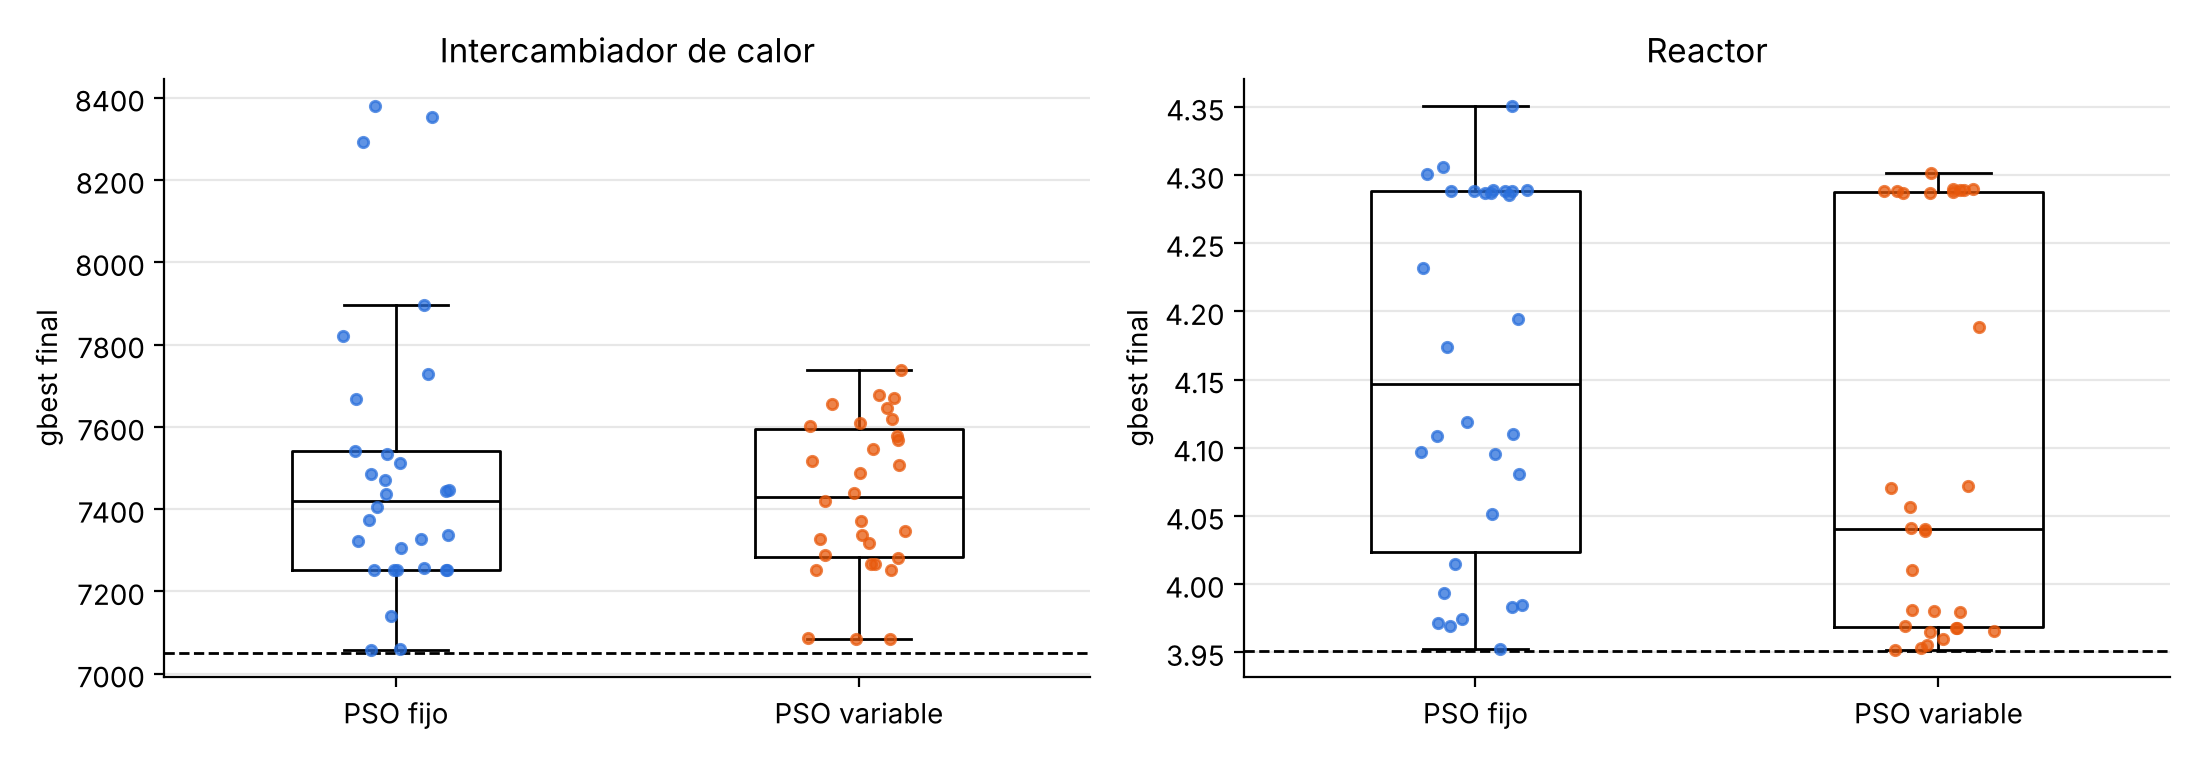
\includegraphics[width=\textwidth]{figuras/distribucion_final.png}
\caption{gbest final de cada una de las 30 ejecuciones por versión. Cada punto es una ejecución; la caja marca los cuartiles y la línea discontinua el óptimo reportado en el libro.}
\label{fig:distribucion}
\end{figure}

En el reactor los resultados no se reparten de forma continua, sino que forman dos grupos. Uno está cerca del óptimo, entre 3.95 y 4.07. El otro está concentrado en un valor casi constante de 4.288, al que llegaron 9 ejecuciones de cada versión. Al revisar las soluciones de este segundo grupo encontramos que en todas $x_1$ está en su cota inferior (0.1) y $x_2$ vale alrededor de 8. En las mejores soluciones, en cambio, el reparto es más equilibrado: $x_1 \approx 6.4$ y $x_2 \approx 2.3$. Es decir, el segundo grupo es un mínimo local en el que la primera rama del problema queda ``apagada'' y toda la reducción del objetivo se obtiene a través de $x_2$. En ambos tipos de solución las cuatro restricciones se cumplen con igualdad, así que el enjambre está pegado a la frontera de la región factible, y para pasar de un mínimo al otro tendría que cambiar varias variables a la vez sin salirse de ella. Una vez que el enjambre cae ahí, ninguna de las dos versiones logra salir. Esto explica que la desviación estándar del reactor sea parecida en ambas versiones: las dos caen en este mínimo con la misma frecuencia. La diferencia entre ellas está en las ejecuciones que no caen en él, donde la versión variable termina más cerca del óptimo (Figura~\ref{fig:distribucion}, derecha).

En el intercambiador los resultados están más dispersos y no hay un mínimo local tan marcado, aunque cinco ejecuciones de la versión fija terminaron entre 7251 y 7252. Las mejores soluciones de cada versión se parecen a la del libro en las temperaturas, pero no tanto en las áreas:
\begin{align*}
\mathbf{x}_{\text{libro}}    &= (579.31,\ 1359.97,\ 5109.97,\ 182.01,\ 295.60,\ 217.98,\ 286.42,\ 395.60), \\
\mathbf{x}_{\text{fija}}     &= (507.53,\ 1278.21,\ 5272.44,\ 175.70,\ 289.10,\ 224.30,\ 286.60,\ 389.10), \\
\mathbf{x}_{\text{variable}} &= (530.01,\ 1106.43,\ 5447.37,\ 177.75,\ 282.11,\ 222.25,\ 295.65,\ 382.11).
\end{align*}
Las tres soluciones tienen un área total muy parecida, pero la reparten de forma distinta entre los intercambiadores: la versión variable, por ejemplo, usa un segundo intercambiador más pequeño y un tercero más grande. Esto sugiere que cerca del óptimo la función objetivo es muy plana en ciertas direcciones, porque se puede quitar área a un equipo y pasársela a otro casi sin cambiar el total. En una superficie así el enjambre avanza muy despacio, lo que ayuda a explicar por qué la media se queda lejos del óptimo.

%%%%%%%%%%%%%%%%%%%%%%%%%%%%%%%%%%%%%%%%%%%%%%%%%%%%%
\subsection{Convergencia del gbest}
\label{sec:convergencia}

La Figura~\ref{fig:convergencia} muestra la media y la desviación estándar del gbest en cada iteración, con el eje horizontal en escala logarítmica para que se vean las primeras iteraciones. La Tabla~\ref{tab:evolucion_gbest} da los valores en algunas iteraciones.

\begin{figure}[H]
\centering
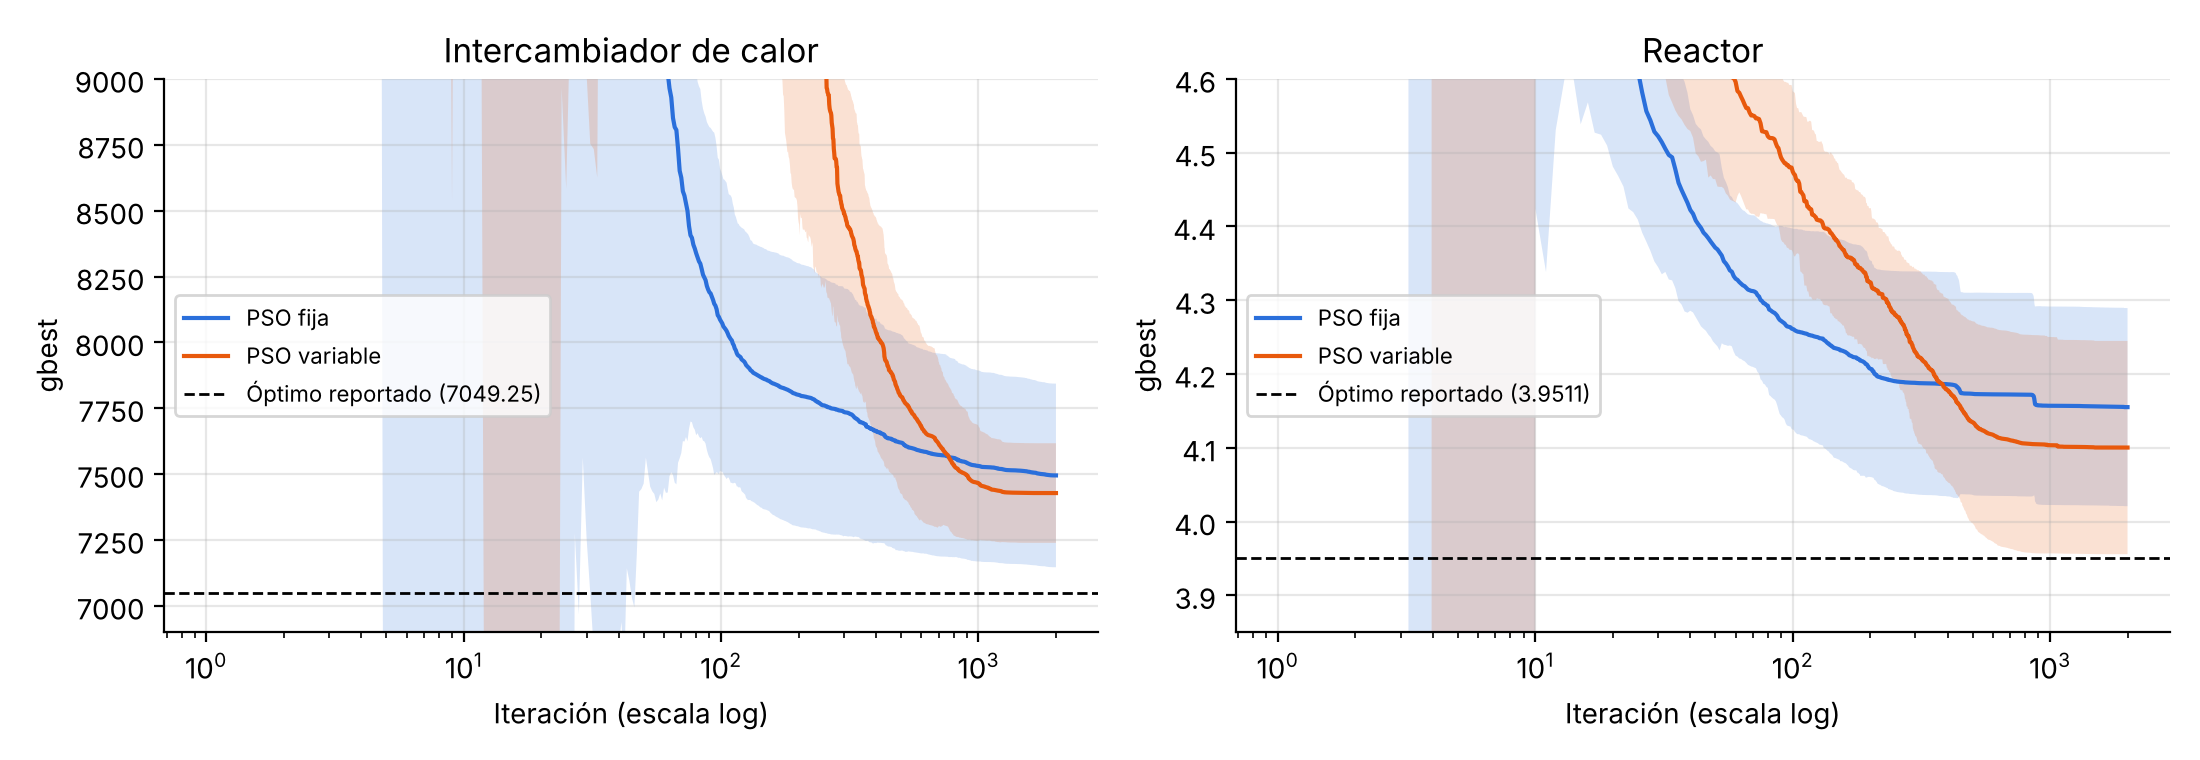
\includegraphics[width=\textwidth]{figuras/convergencia_gbest.png}
\caption{Media (línea) $\pm$ desviación estándar (área sombreada) del gbest en 30 ejecuciones. En las primeras iteraciones la banda es muy ancha porque algunas ejecuciones todavía no tienen soluciones factibles y su gbest incluye la penalización.}
\label{fig:convergencia}
\end{figure}

\begin{table}[H]
\centering
\caption{Media $\pm$ desviación estándar del gbest en distintas iteraciones.}
\label{tab:evolucion_gbest}
\small
\setlength{\tabcolsep}{4pt}
\begin{adjustbox}{max width=\textwidth}
\begin{tabular}{lcccc}
\toprule
 & \multicolumn{2}{c}{Intercambiador} & \multicolumn{2}{c}{Reactor} \\
\cmidrule(lr){2-3}\cmidrule(lr){4-5}
Iteración & Fija & Variable & Fija & Variable \\
\midrule
1    & $9.27\times10^5 \pm 3.62\times10^5$ & $1.17\times10^6 \pm 4.00\times10^5$ & $2.28\times10^5 \pm 1.03\times10^5$ & $2.41\times10^5 \pm 1.06\times10^5$ \\
400  & \textbf{7664.10} $\pm$ 425.77 & 8037.77 $\pm$ 434.22 & 4.1861 $\pm$ 0.1520 & \textbf{4.1779} $\pm$ 0.1243 \\
800  & 7561.69 $\pm$ 376.72 & \textbf{7535.47} $\pm$ 268.46 & 4.1720 $\pm$ 0.1379 & \textbf{4.1058} $\pm$ 0.1476 \\
1200 & 7520.51 $\pm$ 357.58 & \textbf{7437.06} $\pm$ 195.12 & 4.1568 $\pm$ 0.1346 & \textbf{4.1013} $\pm$ 0.1449 \\
2000 & 7495.15 $\pm$ 348.48 & \textbf{7428.22} $\pm$ 189.06 & 4.1552 $\pm$ 0.1343 & \textbf{4.1003} $\pm$ 0.1445 \\
\bottomrule
\end{tabular}
\end{adjustbox}
\end{table}

En la iteración 1 el gbest medio es del orden de $10^5$ a $10^6$ en los dos problemas, lo que confirma que al inicio ninguna partícula es factible. La versión fija sale de la zona penalizada mucho antes: en el intercambiador su gbest baja de 10\,000 en la iteración 39 (mediana de las 30 ejecuciones), mientras que la versión variable tarda hasta la iteración 174. Con $w = 0.9$ y $c_2 = 0.5$ al inicio, las partículas de la versión variable se mueven mucho y casi no se atraen entre sí, así que tardan más en concentrarse en la región factible.

Después de esa primera etapa las curvas se comportan como en la práctica anterior con Rastrigin. La versión fija mejora rápido y después se estanca: en el reactor el gbest medio solo baja de 4.1861 a 4.1552 entre las iteraciones 400 y 2000. La versión variable es más lenta al inicio pero sigue mejorando por más tiempo, y su media queda por debajo de la de la versión fija a partir de la iteración 383 en el reactor y 767 en el intercambiador. Para medir cuándo se estanca cada versión, buscamos en cada ejecución la primera iteración en que el gbest quedó a menos de 0.1\,\% de su valor final. La mediana de esa iteración fue 674 (fija) y 1039 (variable) en el intercambiador, y 300 (fija) y 661 (variable) en el reactor. Después de la iteración 1200 ninguna de las dos versiones mejora de forma apreciable, lo que confirma que 2000 iteraciones fueron suficientes.

%%%%%%%%%%%%%%%%%%%%%%%%%%%%%%%%%%%%%%%%%%%%%%%%%%%%%
\subsection{Diversidad del enjambre}
\label{sec:res_diversidad}

La Figura~\ref{fig:diversidades} muestra las tres medidas de diversidad a lo largo de las iteraciones. Todas se calcularon en el espacio normalizado $[0,1]^8$, así que una diversidad de 0.1 equivale a que las partículas están, en promedio, a una distancia de 10\,\% del rango del centro del enjambre.

\begin{figure}[H]
\centering
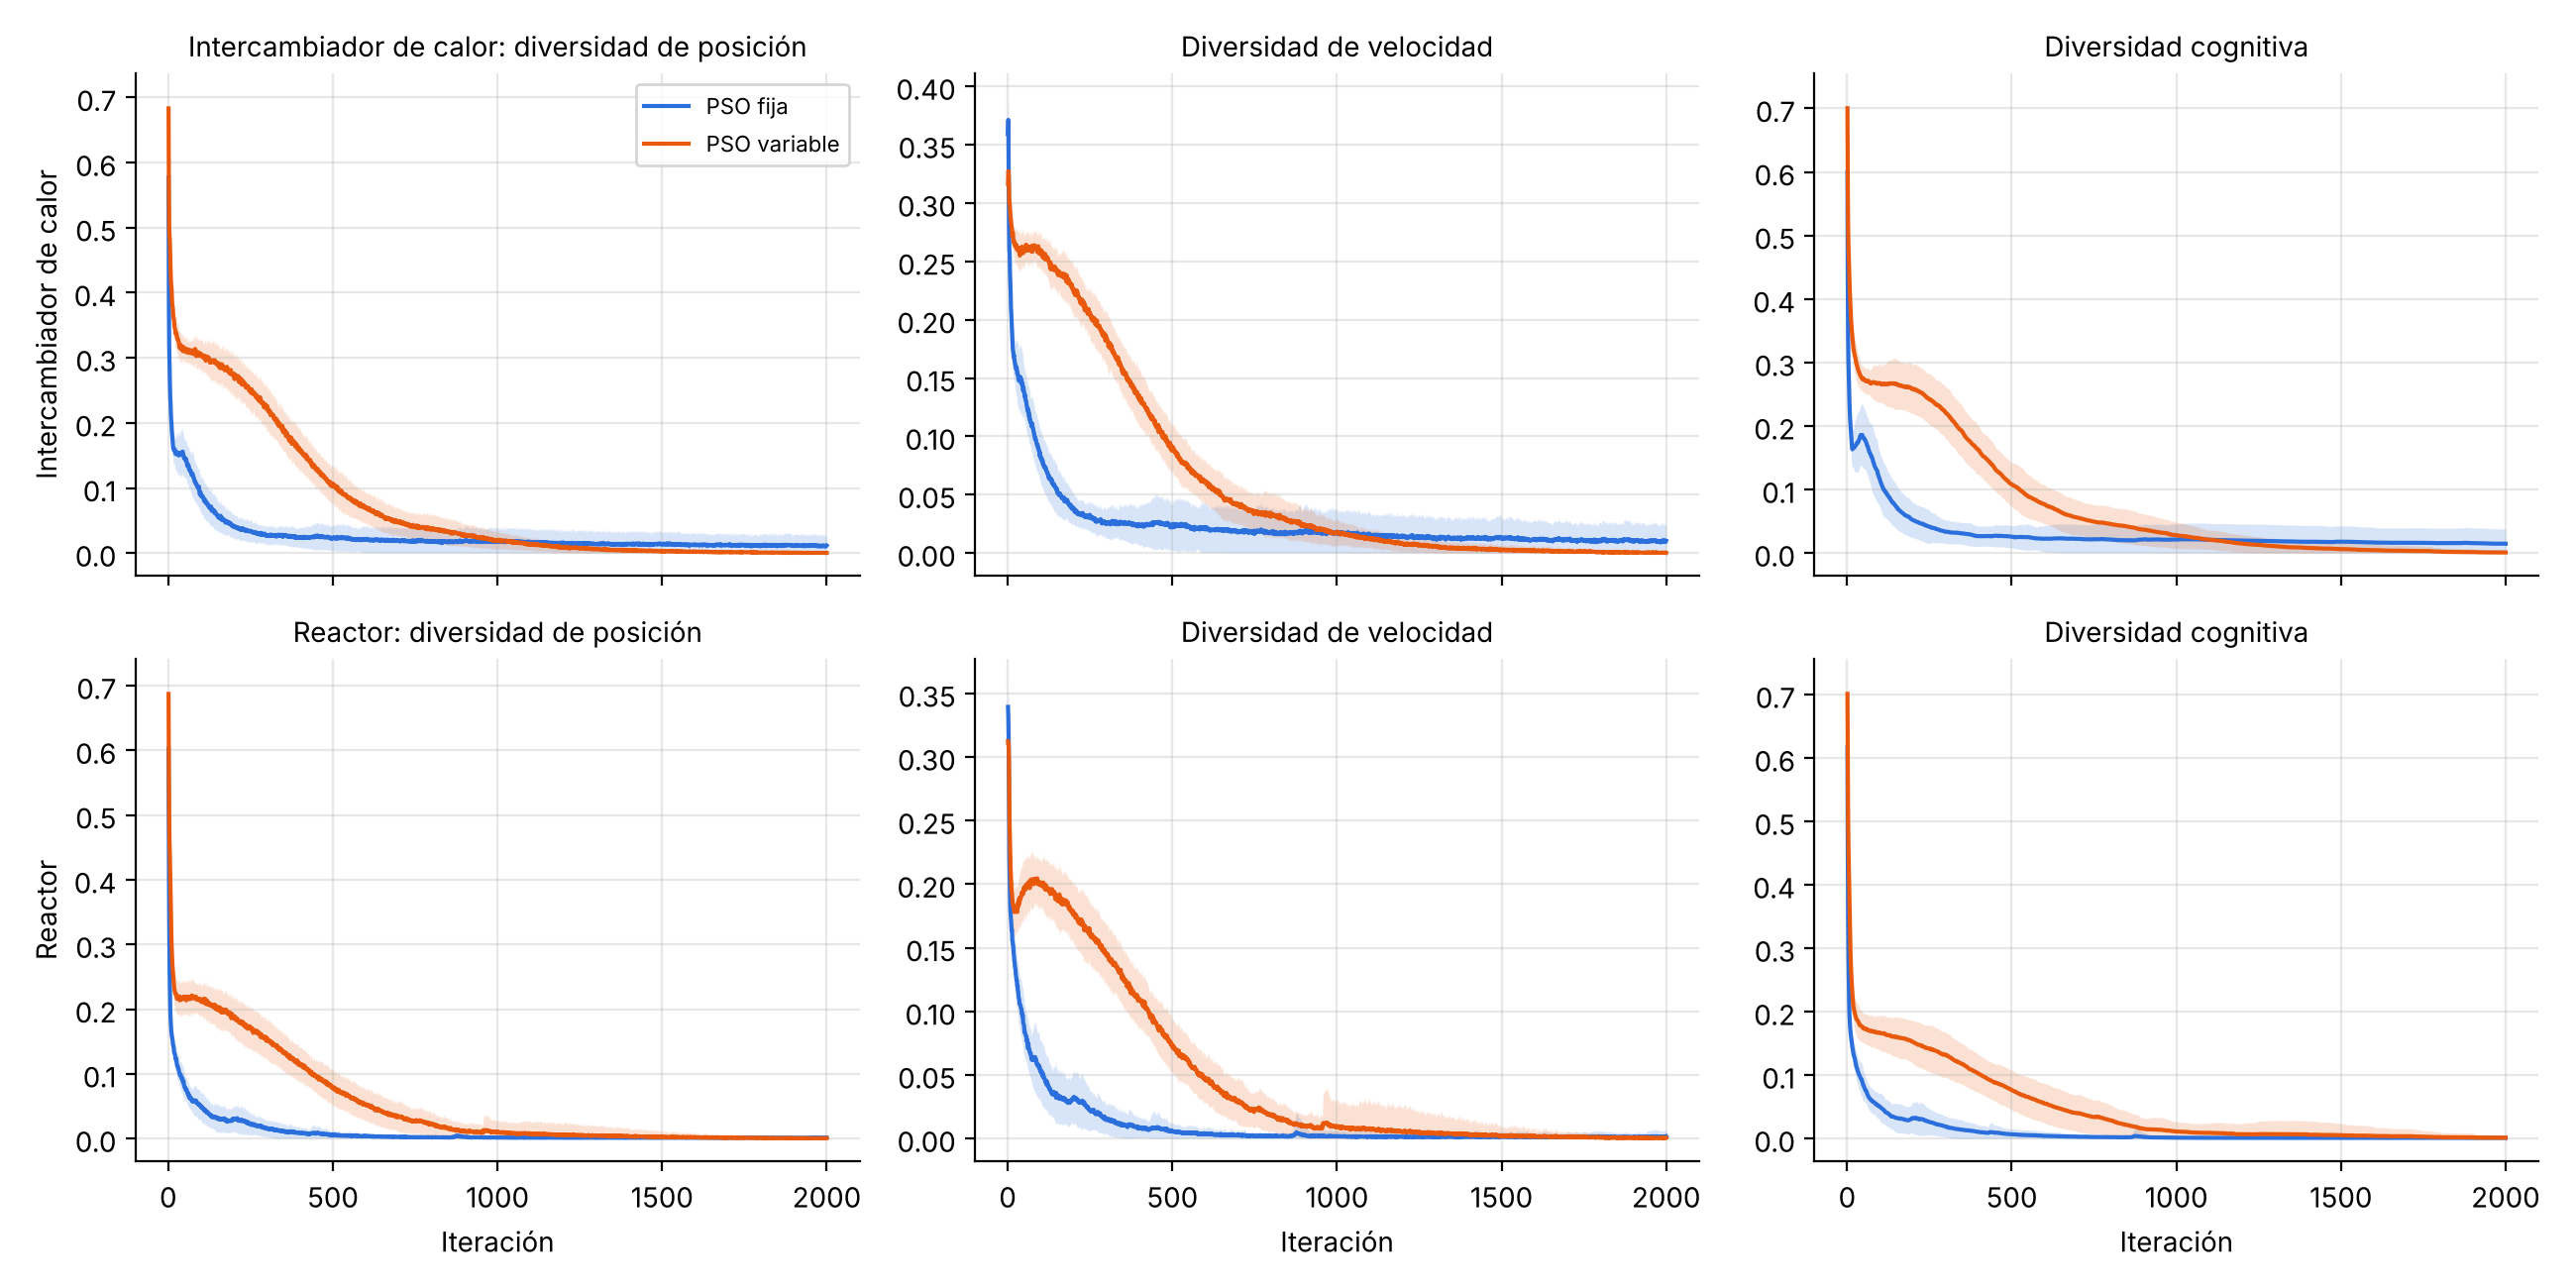
\includegraphics[width=\textwidth]{figuras/diversidades.png}
\caption{Media $\pm$ desviación estándar de la diversidad de posición, de velocidad y cognitiva en 30 ejecuciones. Arriba, intercambiador de calor; abajo, reactor.}
\label{fig:diversidades}
\end{figure}

Las tres medidas siguen el mismo patrón en los dos problemas. En la versión fija la diversidad cae muy rápido en las primeras 100 iteraciones y después se mantiene casi constante y cerca de cero. En la versión variable cae al principio, pero se detiene alrededor de 0.3 en el intercambiador y de 0.2 en el reactor, y a partir de ahí baja de forma gradual durante unas 1000 iteraciones. En la iteración 100, por ejemplo, la diversidad de posición de la versión variable era 0.303 en el intercambiador y 0.211 en el reactor, contra 0.087 y 0.049 de la versión fija.

Esta forma de la curva corresponde a lo que se espera del esquema TVAC. Al inicio $w$ es alto y $c_1$ domina, así que cada partícula se mueve con fuerza y se guía sobre todo por su propio $P_i$; el enjambre se mantiene disperso y explora. Conforme $w$ baja y $c_2$ sube, las partículas se atraen cada vez más hacia $G$ y la diversidad disminuye. La caída coincide en el tiempo con la etapa en la que el gbest de la versión variable mejora más rápido (Figura~\ref{fig:convergencia}), es decir, el enjambre aprovecha lo que encontró durante la exploración.

La diversidad de velocidad y la de posición son casi iguales en forma. Esto tiene sentido porque, sin un término que mueva a las partículas por su cuenta, la velocidad depende de la distancia de cada partícula a $P_i$ y a $G$, que es justo lo que mide la diversidad de posición. La diversidad cognitiva baja un poco más despacio, sobre todo en la versión variable, porque los $P_i$ solo se actualizan cuando una partícula mejora; las posiciones pueden juntarse antes que los recuerdos de cada partícula.

\begin{table}[H]
\centering
\caption{Diversidad en la última iteración (media $\pm$ desviación estándar en 30 ejecuciones).}
\label{tab:diversidad_final}
\small
\setlength{\tabcolsep}{4pt}
\begin{adjustbox}{max width=\textwidth}
\begin{tabular}{llccc}
\toprule
Problema & Versión & Posición & Velocidad & Cognitiva \\
\midrule
\multirow{2}{*}{Intercambiador} & Fija & $1.15\times10^{-2} \pm 1.62\times10^{-2}$ & $1.05\times10^{-2} \pm 1.59\times10^{-2}$ & $1.47\times10^{-2} \pm 2.31\times10^{-2}$ \\
 & Variable & $2.11\times10^{-4} \pm 9.37\times10^{-4}$ & $2.21\times10^{-4} \pm 9.84\times10^{-4}$ & $8.75\times10^{-4} \pm 3.99\times10^{-3}$ \\
\midrule
\multirow{2}{*}{Reactor} & Fija & $1.45\times10^{-3} \pm 4.20\times10^{-3}$ & $1.73\times10^{-3} \pm 5.33\times10^{-3}$ & $1.01\times10^{-3} \pm 2.70\times10^{-3}$ \\
 & Variable & $5.06\times10^{-4} \pm 1.75\times10^{-3}$ & $4.82\times10^{-4} \pm 1.68\times10^{-3}$ & $1.32\times10^{-3} \pm 4.23\times10^{-3}$ \\
\bottomrule
\end{tabular}
\end{adjustbox}
\end{table}

Al final de la ejecución la situación se invierte (Tabla~\ref{tab:diversidad_final}). La versión variable termina con una diversidad menor que la fija, porque en las últimas iteraciones $w = 0.4$ y $c_2 = 2.5$, y todo el enjambre se concentra en un solo punto. En el intercambiador la diferencia es de dos órdenes de magnitud. En las dos versiones la desviación estándar es mayor que la media, lo que indica que la mayoría de las ejecuciones termina con diversidad casi nula y unas pocas mantienen partículas separadas. En la versión fija del intercambiador, la diversidad de posición se quedó alrededor de 0.01 desde la iteración 1000 hasta el final, y en ese mismo tramo el gbest siguió bajando poco a poco (de 7520 a 7495 entre las iteraciones 1200 y 2000). Con $w = 0.7298$ constante, algunas partículas no terminan de detenerse y siguen refinando la solución muy lentamente.

%%%%%%%%%%%%%%%%%%%%%%%%%%%%%%%%%%%%%%%%%%%%%%%%%%%%%
\subsection{Prueba de Wilcoxon}
\label{sec:res_wilcoxon}

La Tabla~\ref{tab:wilcoxon} reporta la prueba de rangos con signo de Wilcoxon entre la versión fija y la variable, aplicada a los valores de la última iteración. Recordemos que con $n = 30$ el valor de $T$ esperado cuando no hay diferencia es 232.5.

\begin{table}[H]
\centering
\caption{Prueba de Wilcoxon pareada (bilateral, $\alpha = 0.05$) entre PSO fijo y PSO variable, sobre los valores de la última iteración.}
\label{tab:wilcoxon}
\small
\setlength{\tabcolsep}{4pt}
\begin{adjustbox}{max width=\textwidth}
\begin{tabular}{llccccc}
\toprule
Problema & Métrica & Mediana fija & Mediana variable & $T$ & Valor $p$ & ¿Diferencia? \\
\midrule
\multirow{4}{*}{Intercambiador} & gbest & 7420.62 & 7430.49 & 232 & 1.000 & No \\
 & Div. posición & $5.56\times10^{-3}$ & $1.51\times10^{-11}$ & 23 & $1.19\times10^{-6}$ & Sí \\
 & Div. velocidad & $4.08\times10^{-3}$ & $3.04\times10^{-11}$ & 25 & $1.68\times10^{-6}$ & Sí \\
 & Div. cognitiva & $5.79\times10^{-3}$ & $8.31\times10^{-11}$ & 43 & $2.37\times10^{-5}$ & Sí \\
\midrule
\multirow{4}{*}{Reactor} & gbest & 4.1465 & 4.0405 & 130 & 0.035 & Sí \\
 & Div. posición & $1.97\times10^{-4}$ & $1.68\times10^{-8}$ & 82 & $1.34\times10^{-3}$ & Sí \\
 & Div. velocidad & $2.31\times10^{-4}$ & $1.11\times10^{-8}$ & 88 & $2.19\times10^{-3}$ & Sí \\
 & Div. cognitiva & $2.08\times10^{-4}$ & $1.39\times10^{-8}$ & 99 & $5.01\times10^{-3}$ & Sí \\
\bottomrule
\end{tabular}
\end{adjustbox}
\end{table}

En el intercambiador no hay diferencia significativa en el gbest final. El estadístico $T = 232$ es prácticamente el valor esperado si las dos versiones fueran equivalentes, y el valor $p$ es 1.000. Al comparar ejecución por ejecución, la versión variable fue mejor en 13 de las 30 parejas y la fija en 17, y las diferencias a favor de cada una tienen tamaños parecidos. La ventaja de la versión variable en la media (Tabla~\ref{tab:gbest_final}) no se refleja en la prueba porque Wilcoxon trabaja con rangos: las tres ejecuciones malas de la versión fija cuentan como tres diferencias grandes, pero no pesan más que su rango.

En el reactor la diferencia sí es significativa ($T = 130$, $p = 0.035$) a favor de la versión variable, que fue mejor en 21 de las 30 parejas. El valor $p$ está cerca del umbral de 0.05, así que la evidencia es moderada. Además, como vimos en la Sección~\ref{sec:res_distribucion}, la ventaja viene de las ejecuciones que no cayeron en el mínimo local de 4.288; en las que sí cayeron, las dos versiones terminan en el mismo valor.

En las tres medidas de diversidad la diferencia es significativa en los dos problemas, siempre con la versión variable terminando más concentrada. En el intercambiador las medianas de la versión variable son del orden de $10^{-11}$, lo que significa que en la mayoría de las ejecuciones todas las partículas terminaron prácticamente en el mismo punto. Estas pruebas confirman de forma estadística lo que se observa en la Figura~\ref{fig:diversidades}: el esquema TVAC cumple su propósito de pasar de un enjambre disperso a uno completamente concentrado, mientras que con coeficientes fijos el enjambre converge pronto pero no termina de cerrarse del todo.
